\begin{frame}
\frametitle{Implementation}
We choose several representative LSH schemes, implement them and compare their performance.
\begin{multicols}{2}
\begin{itemize}
	\item Basic LSH
	\item LSH Forest
	\item Multi-ProbeLSH
	\item Bayesian LSH
\end{itemize}
\end{multicols}

\textbf{Dataset}. We use MNIST\footnote{http://yann.lecun.com/exdb/mnist/} to evaluate the algorithms. We choose 50 dimensions of the original $28\times28$ images with largest variances as ~\cite{gan2012locality} does. Ground truth are got by linear scan in the training set with Euclidean distance.
\end{frame}

\begin{frame}
	\frametitle{Experiment Settings}
	\begin{table}
		\begin{tabular}{ccccc}
			\hline
			Algorithm & Basic & LSHForest & MultiProbe & Bayesian \\ \hline
			\#compounds & 8 & 25 & 8 & \\\hline
			$w$ & 8 & 1 & 8 & \\\hline
			$T$ & - & - & 16 & - \\ \hline
		\end{tabular}
	\end{table}
\end{frame}

\begin{frame}[allowframebreaks]
\frametitle{Error Ratio}
Error ratio indicates the accuracy of LSH's results and the ground truth.
Error ratio is close to 1 means this LSH scheme successfully find the nearest neighbors.
	\begin{equation}
		\text{Error Ratio}=\frac{1}{N}\frac{1}{K}\sum_{n=1}^{N}\sum_{i=1}^{K}\frac{d(q, p_{lsh}^{(i)})}{d(q, p_{label}^{(i)})}
	\end{equation}
We use $K=20$.

\pagebreak
\begin{figure}
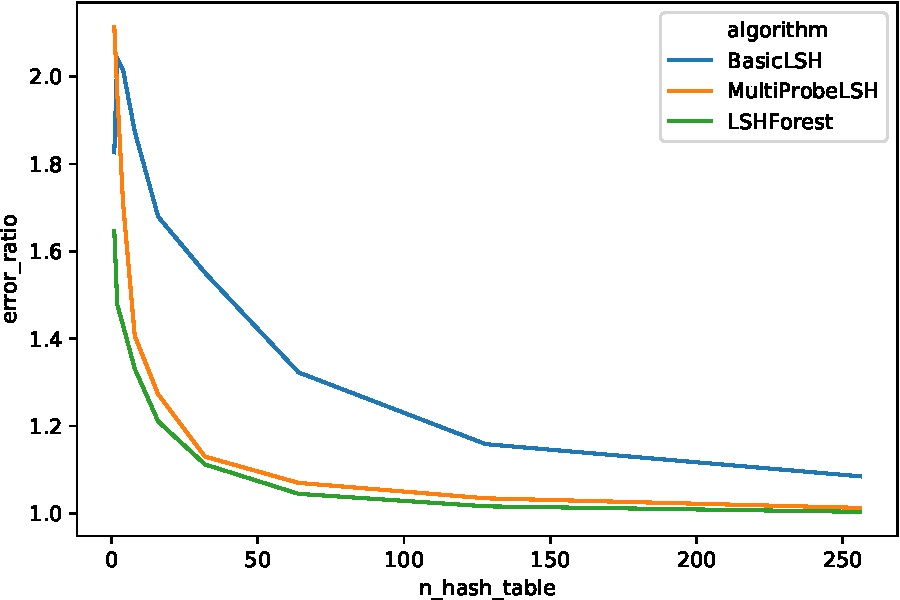
\includegraphics[width=0.8\textwidth]{figures/error_ratio}
\end{figure}
\end{frame}

\begin{frame}[allowframebreaks]
\frametitle{Recall}
Recall shows how many nearest neighbors are found by LSH.
\begin{equation}
	\text{Recall}=\frac{|A_{lsh}\cap A_{label}|}{|A_{label}|}
\end{equation}
\pagebreak
\begin{figure}
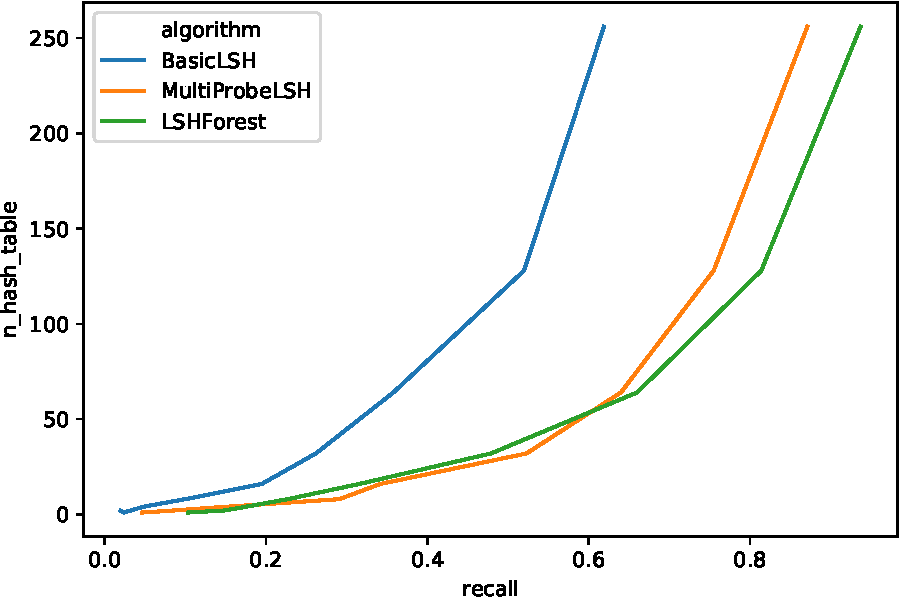
\includegraphics[width=0.8\textwidth]{figures/recall}
\end{figure}
\end{frame}

\begin{frame}[allowframebreaks]
\frametitle{Time Usage}
\begin{figure}
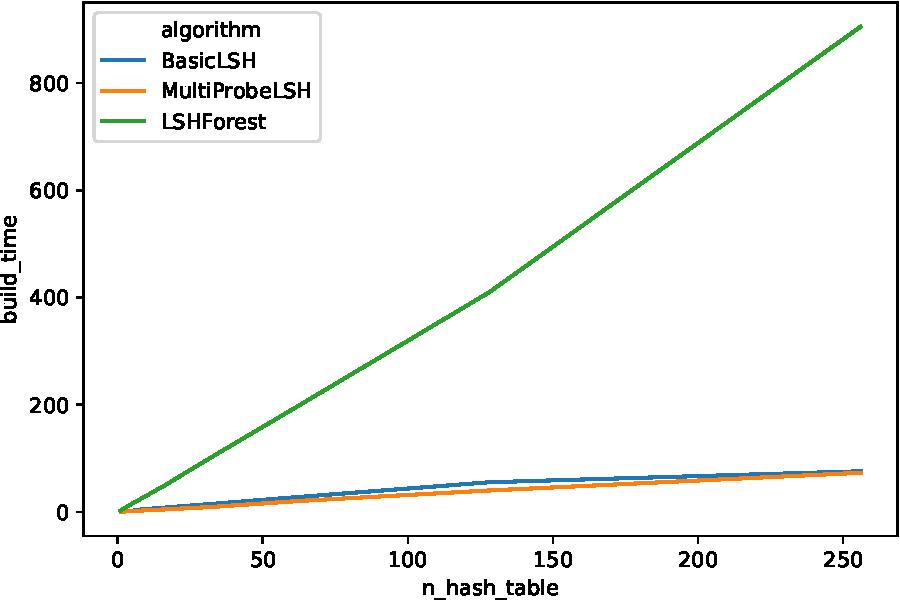
\includegraphics[width=0.8\textwidth]{figures/build_time}
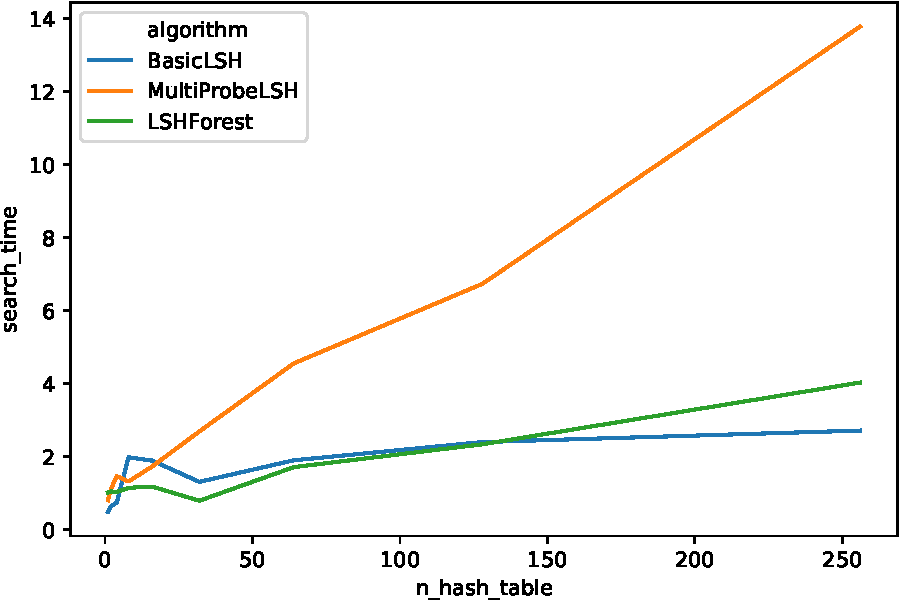
\includegraphics[width=0.8\textwidth]{figures/search_time}
\end{figure}
\end{frame}

\begin{frame}
\frametitle{Candidate Number}
\vspace{-1em}
$$
c/n=\frac{\# candidates}{\# train\ samples}
$$
\vspace{-1em}
\begin{figure}
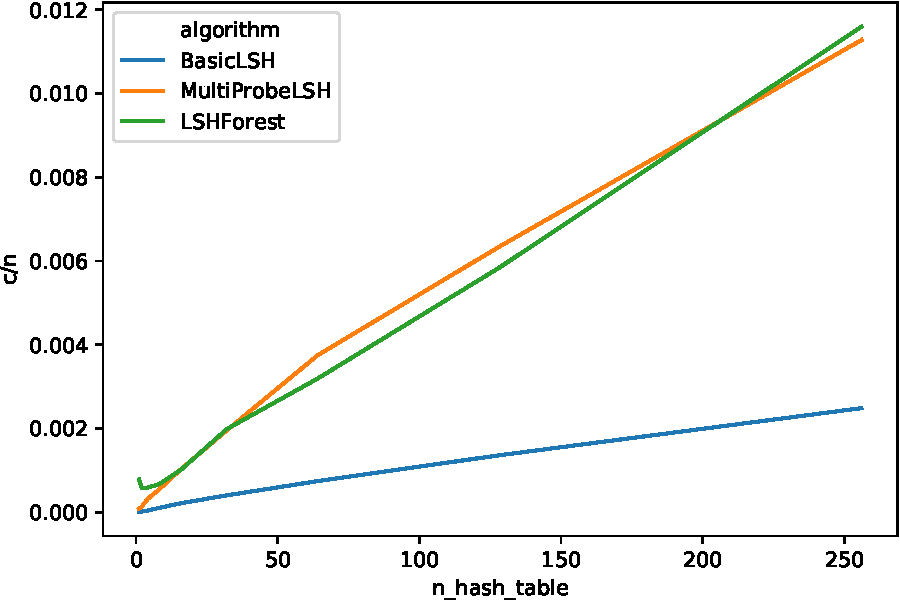
\includegraphics[width=0.8\textwidth]{figures/c_n}
\end{figure}
\end{frame}

\begin{frame}
\frametitle{Observations}
\begin{itemize}
	\item LSHForest and MultiProbeLSH return more candidates with the same number of hash tables. Therefore they have better error ratio and recall than BasicLSH
	\item MultiProbeLSH takes most time in searching because it has to determine the probe sequence at every query.
	\item LSHForest suffers from long build time, especially when there are many hash tables.
\end{itemize}	
\end{frame}


